\documentclass[12pt]{article}
\usepackage[margin=1.1in]{geometry}
\usepackage{amsmath,amssymb}
\usepackage{booktabs,multirow}
\usepackage{graphicx}
\usepackage{natbib}
\usepackage{setspace}
\usepackage[hidelinks]{hyperref}
\usepackage{caption}
\newcommand{\champForecastLL}{0.324}
\newcommand{\champForecastAcc}{86.2}
\newcommand{\champContestedAcc}{85.1}
\newcommand{\champAPRE}{0.48}
\newcommand{\incForecastLL}{0.348}
\newcommand{\champGain}{0.024}
\newcommand{\champCongressoutLL}{0.643}
\newcommand{\majorityCongressoutLL}{0.617}
\newcommand{\gbRawForecastLL}{0.803}
\newcommand{\prospectiveVoneLL}{0.331}
\newcommand{\prospectiveVoneAcc}{85.7}
\newcommand{\prospectiveVtwoLL}{0.332}
\newcommand{\prospectiveVtwoAcc}{86.8}
\newcommand{\prospectiveN}{9,451}
\newcommand{\regimeAbestLL}{0.153}

% auto-generated context
\newcommand{\ukRoll}{1235}
\newcommand{\ukDate}{2024-12-20}
\newcommand{\ukCut}{3.44}
\newcommand{\ukDiscrim}{-1.11}
\newcommand{\ukYeaShare}{92}
\newcommand{\ukNPred}{400}


\title{Reading the Bills: Text, Votes, and the\\ Measurement of Congress}
\author{Andrew B.\ Hall\thanks{Stanford University. Replication materials,
including the full pipeline, model registry, pre-registered experiment
ledger, and session logs of the AI-assisted development process, are
available in the project repository. Every statistic and figure is
generated programmatically from the analysis code's output files; no
number is transcribed by hand.}}
\date{Draft: July 2026 --- preliminary, comments welcome}

\begin{document}
\maketitle
\onehalfspacing

\begin{abstract}
\noindent Political science measures Congress with models that predict
rollcall votes but do not read the bills being voted on. We build an
open benchmark on 10.6 million voting decisions and a vote-prediction
ensemble whose modern language-model encoders do read them, and
establish three results. \emph{First, the approach outperforms
existing ones}: on identical held-out votes it beats DW-NOMINATE on
the classification literature's own statistic, with the gains
concentrated in precisely the members one-dimensional scaling
famously mis-measures (Ron Paul's geometric mean probability rises
from \paulGMPnom{} to \paulGMPours); on strictly future votes it
reaches \champForecastAcc\% accuracy, far beyond both classical
models and the 2011--2016 text-based literature, with a hash-pinned
frozen artifact scored on votes cast after it was finalized.
\emph{Second, reading the text is what lets the model anticipate
protest voting}: on a storied majority-splitting vote, the same
architecture without text misreads the coalition entirely, while the
text-reading model prices the right-flank revolt member by member,
naming all five likeliest defectors correctly; across
\protRC{} held-out majority-side rollcalls, text raises
within-vote defection detection from \protAUCnotext{} to
\protAUCtext{} AUC. \emph{Third, text predicts where a bill will cut
the chamber before anyone votes}: on \cutTestN{} held-out future
rollcalls, text plus metadata locates cutpoints at $r = \cutComboR$
and calls the coalition's direction at \dirCombo\%---a prospective
capability the bill-location literature, which requires realized
votes, has not had. We release the benchmark, models, an interactive
forecaster, and a pre-registered ledger of every experiment, positive
and negative.
\end{abstract}

\section{Introduction}

Nearly everything political science measures about Congress---ideal
points, party unity, issue positions---comes from models of rollcall
votes that treat the bill being voted on as a blank: an indexed event
with parameters, not a text with content \citep{poole1997congress,
clinton2004statistical}. A short literature at the intersection of
machine learning and legislative studies tried to change that with
the text tools of its era \citep{gerrish2011predicting,
kraft2016embedding}, and the measurement literature has since pushed
on the classical model from many directions---unpredictable voters
\citep{lauderdale2010unpredictable}, issue-specific dimensions
\citep{lauderdale2014scaling, crespin2010dimensions}, massive-data
estimators \citep{imai2016fast}, machine learning as measurement
\citep{bonica2018inferring}, and, most recently, bespoke models for
the members whom one-dimensional scaling visibly mis-measures:
extremists who vote with the opposite pole \citep{duckmayr2023ends}
and majority members who cast protest votes against bills they prefer
\citep{fowler2026protest}. Modern language models can now read
legislative text incomparably better than anything available to that
program. This paper asks what that buys the measurement of Congress,
and gives a three-part answer.

\textbf{One: the approach outperforms existing ones}
(Section~\ref{sec:outperform}). On an open benchmark of 10.6 million
voting decisions (101st--119th Congresses), our models beat the
classical toolkit in both of its own arenas. In the psychometric
completion setting, an expressive spatial model beats frozen
DW-NOMINATE member by member on the NOMINATE literature's own
statistic---and the improvements concentrate exactly in the hard
cases that motivated a decade of bespoke scaling models. In genuine
forecasting, a text-reading ensemble reaches \champForecastAcc\%
accuracy on strictly future votes (\champContestedAcc\% on contested
votes), where the 2011--2016 text models, honestly re-evaluated,
never beat a simple table of member voting rates. A frozen,
hash-pinned artifact scored only on votes cast after its finalization
certifies that these numbers are not artifacts of researcher
iteration.

\textbf{Two: reading the bill is what lets the model anticipate
protest voting} (Section~\ref{sec:protest}). Protest voting---majority
members defecting on bills they arguably prefer---is the newest front
in the scaling literature \citep{fowler2026protest, duckmayr2023ends}.
We show the phenomenon is \emph{predictable in advance}, and that the
text is what does the work: member history tells the model who sits
on a bill's losing flank, but only the text tells it \emph{which
bills} provoke a flank revolt. Without text, the December 2024
shutdown-averting continuing resolution looks like a routine
majority-party bill; reading it, the model recognizes a
bipartisan leadership deal, snaps Democratic support to
near-certainty, and prices the right-flank revolt member by
member---its five likeliest defectors in the chamber all voted nay.
Across every majority-side rollcall in the holdout window, text
raises within-vote defection detection from \protAUCnotext{} to
\protAUCtext{} AUC.

\textbf{Three: text predicts where a bill will cut the chamber}
(Section~\ref{sec:cutpoints}). The bill-location literature estimates
proposal and status-quo positions from realized votes and
cosponsorships \citep{peress2013estimating, richman2011parties}; it
cannot locate a bill that has not been voted on. We show that a
bill's text does: on held-out future rollcalls, text plus pre-vote
metadata predicts realized cutpoint locations at $r = \cutComboR$ and
coalition direction at \dirCombo\%, and the division of labor is
itself informative---institutional metadata pins \emph{where} a vote
cuts, the acting legislator's party supplies a default side, and
content tells the model when the default is wrong. An interactive
forecaster operationalizes the result: paste a bill, get a predicted
cutpoint and a member-by-member forecast.

Everything else this exercise produced---evaluation-regime audits,
negative results with diagnosed mechanisms, the limits of member
history across majority transitions---is documented in the appendices
and repository; Section~\ref{sec:limits} states the two boundaries a
user of these methods must know.

\section{Benchmark, Models, and Definitions}
\label{sec:setup}

\textbf{Task and data.} We predict individual voting decisions: given
everything observable before a rollcall, each member's probability of
voting yea, conditional on a recorded yea or nay. The panel is every
such decision in the 101st--119th Congresses from Voteview
\citep{lewis2026voteview}; bill-side information (titles, dated
summary versions, sponsors, amendment records) comes from government
BILLSTATUS files, which begin with the 108th Congress. All
forecasting results use the text-era congresses (108th--119th);
earlier congresses enter only the no-text completion fits. Splits are
deterministic and content-hashed; the harness strips labels before
models see evaluation rows; the feature-timing audit is
Appendix~\ref{app:audit}.

\textbf{Evaluation.} Regimes with progressively stricter information
constraints: \emph{completion} (random votes held out, same-rollcall
votes observable---the psychometric setting), \emph{temporal forecast}
(each congress-chamber's final ten percent of rollcalls by date), and
\emph{prospective} (hash-pinned frozen artifacts scored only on votes
cast afterward, per the reusable-holdout logic of
\citealp{dwork2015holdout}). Metrics are the field's: correct
classification, APRE, and geometric mean probability
\citep{carroll2013structure}, with log loss ($= -\log \mathrm{GMP}$)
as the primary scoring rule.

\textbf{Models.} The forecasting champion is a logistic blend of
two-tower networks: member embeddings meet rollcall parameters
amortized from pre-vote text (vote question, description, latest
pre-vote bill summary) by sentence encoders and a deep head, anchored
on member-by-question empirical rates, calibrated on a temporal
internal slice of training data. Its no-text counterpart---the
identical architecture with the text deleted---is the counterfactual
throughout. The classical comparators are logistic ideal points, a
frozen-DW-NOMINATE model, and faithful reimplementations of the
2011--2016 text-based models. Full specification:
Appendix~\ref{app:spec}; development followed a pre-registered
experiment ledger (Appendix~\ref{app:ledger}).

\textbf{Definitions.} The spatial fits estimate $P(\text{yea}) =
\sigma(a_v x_i + b_v + c_i)$ per chamber-congress (party-sign
initialized); a rollcall's \emph{average-member cutpoint} is
$-(b_v + \bar c)/a_v$, reported when $|a_v| \geq 0.35$ on the fitted
scale, with \emph{direction} $\mathrm{sign}(a_v)$. All derived
quantities are conditional on the realized rollcall agenda.

\section{Point One: It Outperforms Existing Approaches}
\label{sec:outperform}

The classical toolkit sets two bars, and the approach clears both.

\textbf{Against the canonical measure, on its own statistic.} In the
completion regime---the setting in which ideal-point models are
traditionally assessed---an eight-dimensional spatial model reaches
GMP \regimeAbestGMP{} (\regimeAbestAcc\% classification) on held-out
votes, against \regimeAnominateGMP{} for frozen DW-NOMINATE with
estimated rollcall parameters (full ladder:
Appendix Table~\ref{tab:regimeA}). Figure~\ref{fig:membergmp} makes
the comparison member by member on identical held-out votes, and the
\emph{location} of the margin is the finding. For the typical member,
DW-NOMINATE is nearly unimprovable (median GMP \memberGMPmedNom{}
versus \memberGMPmedOurs; the richer model is higher for
\memberGMPshare\% of members). The large gains sit precisely on the
members the past decade of scaling research built bespoke models to
rescue---Ron Paul (\paulGMPnom{} $\rightarrow$ \paulGMPours), Justin
Amash, Thomas Massie, Dennis Kucinich: the ends-against-the-middle
and protest voters of \citet{duckmayr2023ends} and
\citet{fowler2026protest}, absorbed here by one flexible model.
Convergent validity holds throughout: positions correlate with
DW-NOMINATE at $r = .98$ and with Nokken--Poole per-congress scores
\citep{nokken2004congressional} at $r = \npRmin$--$\npRmax$.

\begin{figure}[t]
\centering
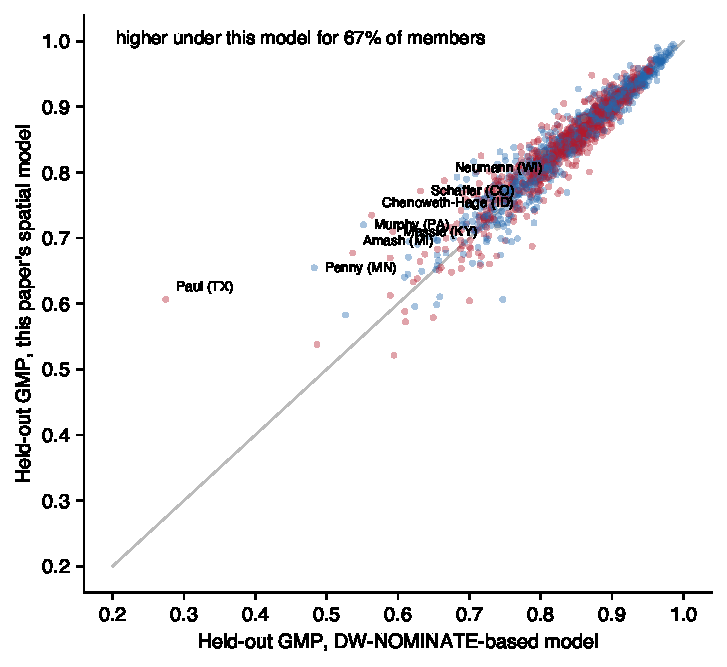
\includegraphics[width=.68\linewidth]{figures/member_gmp.pdf}
\caption{\textbf{The killer comparison for point one.} Every member's
geometric mean probability on identical held-out votes: this paper's
spatial model (vertical) against the classical frozen-DW-NOMINATE
model (horizontal). The typical member sits on the diagonal---the
classical model is excellent---and the large gains are exactly the
literature's canonical hard cases (labeled). Blue: Democrats; red:
Republicans.}
\label{fig:membergmp}
\end{figure}

\textbf{Against everything, in genuine forecasting.}
Table~\ref{tab:regime} reports the temporal-forecast horse race: the
ensemble reaches \champForecastLL{} log loss
(GMP \champForecastGMP; \champForecastAcc\% accuracy,
\champContestedAcc\% on contested votes, APRE \champAPRE) on
\forecastTestN{} strictly future votes. The 2011--2016 text-based
architectures, reimplemented faithfully and given modern courtesies,
never beat the member-history count table under proper scoring
(Appendix Table~\ref{tab:lit}); the raw Gerrish--Blei-style model is
worse than predicting the base rate. Paired rollcall-cluster
bootstraps put the ensemble's margin over its own strongest
components at $[\pairedDeltaOneLo, \pairedDeltaOneHi]$ log loss---the
gains are not clustering artifacts. And the numbers survive the only
test no iteration can touch: a predecessor artifact frozen June 12,
2026 scored \prospectiveVoneLL{} log loss (\prospectiveVoneAcc\%
accuracy) on the \prospectiveN{} member-vote decisions Congress cast
after its data snapshot---\postFreezeLL{} on the strictly post-freeze
subset---matching its development performance
(Table~\ref{tab:prospective}); the ensemble's own post-freeze ledger
accumulates.

\begin{table}[t]
\centering
\caption{The temporal-forecast horse race (test log loss and accuracy
under identical evaluation; congress-out transfer in the right panel
foreshadows Section~\ref{sec:limits}).}
\label{tab:regime}
\begin{tabular}{lcccc}
\toprule
Information used & \multicolumn{2}{c}{Temporal forecast} & \multicolumn{2}{c}{Congress-out} \\
\midrule
Party history only & 0.466 & 76.6 & 0.693 & 57.1 \\
Member history only & 0.459 & 76.0 & 0.693 & 57.1 \\
Rollcall metadata only & 0.511 & 72.3 & 0.717 & 58.6 \\
Text + metadata (no member history) & 0.464 & 77.8 & 0.741 & 64.4 \\
Text + metadata + member history & 0.411 & 80.1 & 0.720 & 59.3 \\
+ modern encoder, deep head, calibration & 0.348 & 85.2 & 0.670 & 61.6 \\
+ ensemble (final) & 0.324 & 86.2 & 0.643 & 62.1 \\
\bottomrule
\end{tabular}

\end{table}

\begin{table}[t]
\centering
\caption{Frozen, hash-pinned artifacts scored on votes cast after
their June 9, 2026 data snapshot (freezes: June 12 and July 3).
Bootstrap 95\% interval for v1 log loss: \prospLLlo--\prospLLhi.}
\label{tab:prospective}
\begin{tabular}{llrrccc}
\toprule
Artifact & Snapshot & Rollcalls & Votes & Log loss & Acc.\ (\%) & AUC \\
\midrule
v1 (emb2-MLP tower) & 2026-06-09 & 43 & 9,451 & 0.331 & 85.7 & 0.924 \\
v2 (three-tower blend) & 2026-06-09 & 43 & 9,451 & 0.332 & 86.8 & 0.921 \\
\bottomrule
\end{tabular}

\end{table}

\section{Point Two: Text Detects Protest Voting}
\label{sec:protest}

Protest voting is the scaling literature's newest problem: majority
members voting against bills they arguably prefer, which
one-dimensional models mis-read as moderation
\citep{fowler2026protest, duckmayr2023ends}. Existing treatments are
retrospective---bespoke likelihoods that reinterpret votes already
cast. We show protest voting is \emph{predictable in advance}, and
that reading the bill is what makes it so.

The mechanism has two parts. Member history identifies \emph{who}
lives on a bill's losing flank---but history alone cannot know which
bills put the flank in revolt, because that depends on what the bill
\emph{is}: a leadership compromise, a bipartisan spending deal, a
suspension-calendar package. That is content, and it is in the text.
Figure~\ref{fig:protest} shows the two models side by side on the
December 2024 American Relief Act---the shutdown-averting continuing
resolution passed 366--34 over a right-flank revolt, deep in the
holdout window. Without text, the architecture prices the vote like a
routine majority bill: Democratic support uncertain, the revolt
invisible. Reading the bill, it recognizes the deal: Democratic
probabilities snap to near one, Republican probabilities slide with
distance from the center, and the five members it considers the
likeliest defectors in the entire chamber---Brecheen, Roy, Massie,
Crane, Biggs---all vote nay.

\begin{figure}[t]
\centering
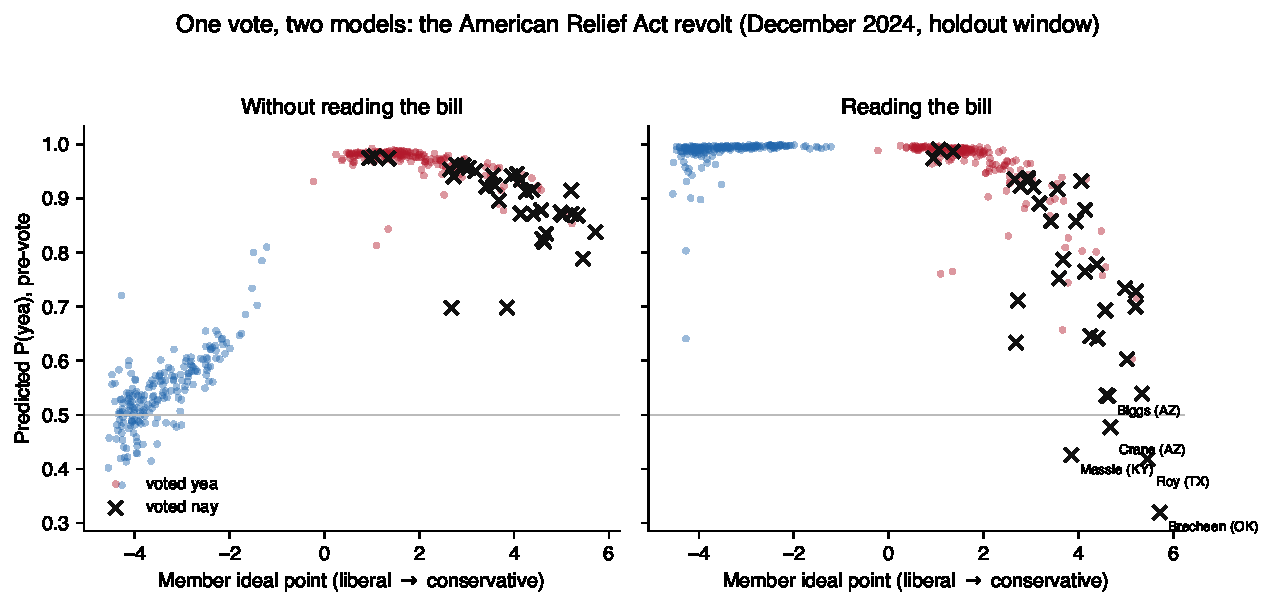
\includegraphics[width=.98\linewidth]{figures/protest_detection.pdf}
\caption{\textbf{The killer comparison for point two.} One
majority-splitting vote (H.R.~10545, December 20, 2024), predicted by
the same architecture without text (left) and with it (right). Dots:
members who voted yea (party-colored); crosses: the 34 nays. Only the
text-reading model locates the revolt---its five likeliest defectors
chamber-wide (labeled) all voted nay.}
\label{fig:protest}
\end{figure}

The episode generalizes. Define the detection task on every held-out
rollcall where a member's party majority voted yea: rank that party's
members by predicted defection probability. Across \protRC{} such
rollcalls with at least three defections (\protN{} defections in
total), the text-reading model achieves a within-vote AUC of
\protAUCtext{} against \protAUCnotext{} for its no-text
counterpart---text converts roughly a fifth of the remaining ranking
errors. Two connections close the loop with the measurement
literature. The members whose \emph{scaling} improves most in
Figure~\ref{fig:membergmp} are the same protest-prone members whose
\emph{defections} the text model prices here: what a one-dimensional
model records as inexplicable moderation is, to a model that reads
the agenda, systematic and forecastable behavior. And the ensemble's
largest remaining residuals---defections incompatible with even the
full behavioral record---are released as a ranked ledger: a sampling
frame, strongly enriched for pressure and defection episodes, for
studying the votes that even text cannot explain.

\section{Point Three: Text Predicts Bill Cutpoints}
\label{sec:cutpoints}

The bill-location literature recovers proposal and status-quo
positions from realized votes and cosponsorship
\citep{peress2013estimating, richman2011parties}---after the fact, by
construction. If bill content organizes coalitions, a bill's text
should locate it \emph{before} anyone votes. It does. For every
rollcall we take the realized cutpoint and direction from the spatial
fits, hold out the final twenty percent of each congress-chamber's
rollcalls, and predict them from strictly pre-vote features.
Figure~\ref{fig:cutpred} and Table~\ref{tab:cutpred} give the result:
on the \cutTestN{} identified held-out rollcalls, text plus metadata
reaches $\mathrm{MAE} = \cutComboMAE$ member-standard-deviations and
$r = \cutComboR$ (no-feature baseline: $\mathrm{MAE} = \cutConstMAE$,
$r = 0$), and calls coalition direction at \dirCombo\%
(majority-direction baseline: \dirConst\%).

\begin{figure}[t]
\centering
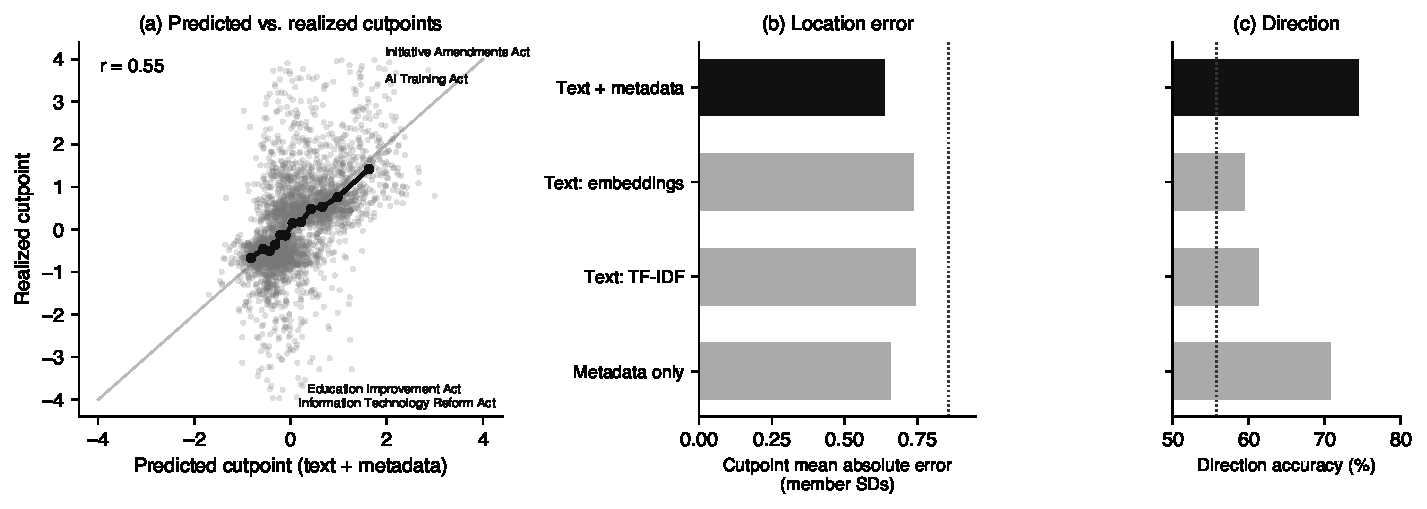
\includegraphics[width=.98\linewidth]{figures/cutpoint_prediction.pdf}
\caption{\textbf{The killer comparison for point three.} Left:
predicted against realized cutpoints for held-out future rollcalls
(text + metadata), landmark bills labeled. Right: error and direction
accuracy by feature set; dotted lines are the no-feature baseline.}
\label{fig:cutpred}
\end{figure}

\begin{table}[t]
\centering
\caption{Predicting held-out rollcalls' cutpoints and directions from
pre-vote features; bottom panel decomposes the text by component.}
\label{tab:cutpred}
\begin{tabular}{lccc}
\toprule
Features & Cutpoint MAE & Cutpoint $r$ & Direction acc.\ (\%) \\
\midrule
Constant & 0.856 & 0.00 & 55.8 \\
Metadata only & 0.657 & 0.48 & 70.8 \\
Text: TF--IDF & 0.742 & 0.43 & 61.3 \\
Text: embeddings & 0.735 & 0.42 & 59.5 \\
Text + metadata & 0.637 & 0.55 & 74.5 \\
\quad question only & 0.763 & 0.41 & 58.2 \\
\quad description only & 0.813 & 0.25 & 57.2 \\
\quad bill summary only & 0.765 & 0.38 & 59.7 \\
\bottomrule
\end{tabular}

\end{table}

The decomposition assigns each input its role. Institutional metadata
(question type, the bill sponsor's and---on amendment votes---the
amender's party, with their interactions) is a formidable baseline:
it pins \emph{where} votes cut ($\mathrm{MAE} = \cutMetaMAE$) and
supplies a default side (\dirMeta\%). Text improves every metric on
top of it, most of all direction (\dirCombo\%) and location
correlation ($\cutMetaR \rightarrow \cutComboR$): the acting
legislator's party says which side a bill is probably on; content
says when that default is wrong, and by how much. Among text
components, the bill summary carries direction and the vote question
carries location. At the term level (interpretable sparse model,
final-passage summaries only), the language of program-building
(\emph{establish}, \emph{grants}, \emph{assistance}, \emph{workers})
is associated with liberal-yea coalitions and the language of
restraint and revision (\emph{rule}, \emph{regulation}, \emph{permit},
\emph{budget}, \emph{injury}) with conservative-yea ones---predictive
associations on a leader-curated agenda, not causal claims. An
interactive forecaster operationalizes the section: paste a
hypothetical bill's text, choose a sponsoring party and chamber, and
receive a predicted cutpoint and member-by-member forecast, with
self-consistency warnings for off-agenda extrapolations
(Appendix~\ref{app:dashboard}).

\section{Two Boundaries}
\label{sec:limits}

Users of these methods must know where they stop, and both boundaries
are measured, not conjectured. \emph{Majority transitions}: at every
House majority flip in the window (none of the placebo transitions),
the procedural-vote component of member history inverts---the
champion's procedural log loss averages \flipProcLL{} across flips
versus \placeboProcLL{} across placebos, while final-passage transfer
is flip-invariant (\flipPassLL{} versus \placeboPassLL;
Appendix Figure~\ref{fig:transitions}). Much of what any vote-based
measure captures on the procedural agenda is institutional role, not
stable preference, and scores estimated in one majority configuration
should cross configurations only with care \citep{bateman2017house}.
\emph{Amendments}: supplying amendments' purpose text makes
prediction worse, not better, in pre-registered, placebo-controlled
experiments; what moves amendment prediction is actor identity (the
amender's party takes direction accuracy from a coin flip to 77
percent). Short purpose text adds nothing once bill identity and
procedural context are modeled---a measured limit on what legislative
language reveals, at least in the representations tested here.

\section{Conclusion}

Reading the bills makes Congress more measurable in three specific
ways: a fit standard that dominates the classical measure exactly
where it struggles, advance detection of the protest voting that
scaling models could previously only reinterpret, and prospective
bill locations that the agenda literature could previously only
estimate in retrospect. The benchmark, the frozen artifacts whose
forecasting claims the future continues to audit, the interactive
forecaster, and a complete ledger of what failed along the way are
released together.

\bibliographystyle{apsr}
\bibliography{references}

\appendix

\section{Additional Tables}
\label{app:tables}

\begin{table}[h]
\centering
\caption{Completion regime (held-out vote completion; same-rollcall
votes observable): the psychometric ladder.}
\label{tab:regimeA}
\begin{tabular}{lcccc}
\toprule
Model & Log loss & Acc.\ (\%) & Contested acc.\ (\%) & APRE \\
\midrule
Constant rate & 0.655 & 63.7 & 50.9 & -0.32 \\
Member rate & 0.629 & 64.9 & 55.2 & -0.28 \\
Party $\times$ rollcall majority & 0.206 & 91.7 & 92.8 & 0.70 \\
Ideal points (1D) & 0.193 & 91.6 & 91.2 & 0.69 \\
DW-NOMINATE logit (frozen scores) & 0.164 & 93.3 & 93.9 & 0.76 \\
Ideal points (2D) & 0.161 & 93.3 & 93.8 & 0.76 \\
Ideal points (8D) & 0.153 & 93.8 & 94.3 & 0.77 \\
\bottomrule
\end{tabular}

\end{table}

\begin{table}[h]
\centering
\caption{The 2011--2016 text-based architectures, reimplemented and
honestly evaluated.}
\label{tab:lit}
\begin{tabular}{lccccc}
\toprule
Model & Fcst.\ LL & Fcst.\ AUC & Fcst.\ cont.\ acc.\ (\%) & Rand.\ LL & Rand.\ AUC \\
\midrule
Constant rate & 0.617 & 0.500 & 52.7 & 0.659 & 0.500 \\
Party $\times$ question rate & 0.466 & 0.805 & 69.8 & 0.504 & 0.797 \\
Member $\times$ question rate & 0.459 & 0.812 & 69.2 & 0.494 & 0.807 \\
NOMINATE $\times$ context logit & 0.532 & 0.740 & 59.6 & 0.587 & 0.713 \\
GB-style spatial (TF-IDF) & 0.803 & 0.689 & 57.6 & 1.054 & 0.687 \\
GB-style spatial (TF-IDF, calibrated) & 0.566 & 0.689 & 57.1 & 0.685 & 0.687 \\
GB-style spatial (mod.\ emb., calibrated) & 0.556 & 0.699 & 55.8 & 0.662 & 0.670 \\
Kraft-style bilinear & 0.497 & 0.790 & 67.2 & 0.522 & 0.794 \\
TF-IDF tower + member offset & 0.411 & 0.860 & 75.0 & 0.448 & 0.854 \\
MiniLM-MLP tower (prior champion) & 0.348 & 0.906 & 84.0 & 0.417 & 0.880 \\
Three-tower blend (champion) & 0.324 & 0.919 & 85.1 & 0.390 & 0.896 \\
\bottomrule
\end{tabular}

\end{table}

\begin{figure}[h]
\centering
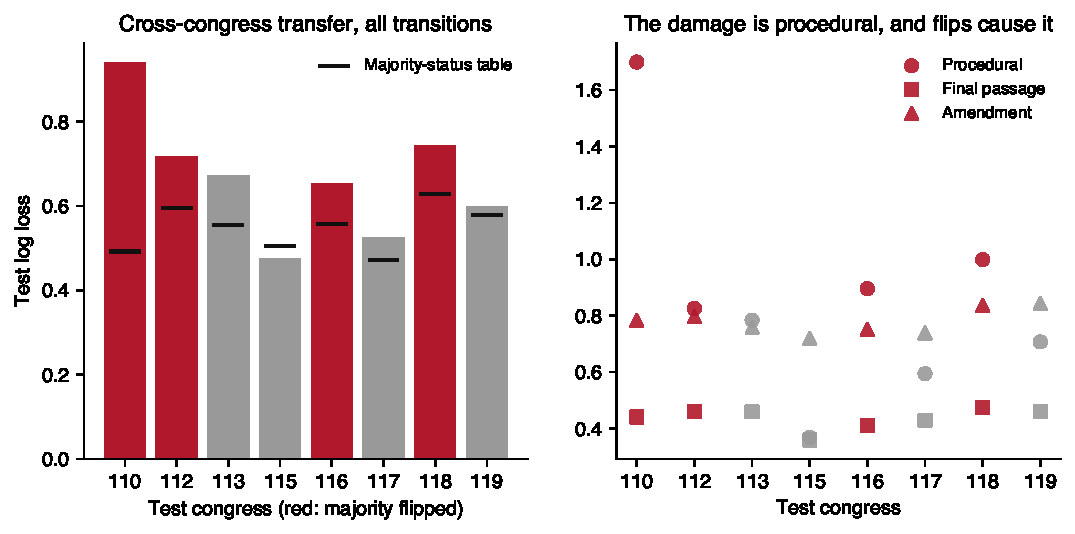
\includegraphics[width=.95\linewidth]{figures/transitions.pdf}
\caption{Majority-transition study: cross-congress transfer at every
House transition (red: flips), overall and by vote type.}
\label{fig:transitions}
\end{figure}

\section{Measurement Provenance}
\label{app:provenance}

Which estimator produces each quantity:
the ensemble produces vote forecasts (pre-vote), the protest-detection
scores (pre-vote), and the out-of-character residual ledger
(in-sample, labeled as such); per chamber-congress spatial fits
produce positions, cutpoints, and directions (from realized votes);
ridge/logistic models on pre-vote features produce the cutpoint
\emph{predictions} of Section~\ref{sec:cutpoints}. An identifiability
remark bounds the enterprise: if two member-rollcall states induce
the same conditional vote distribution given available information,
no measure computed from that information can distinguish them. The
repository's synthetic suite demonstrates the constructive direction:
planted structures are recovered exactly by the models whose held-out
scores improve.

\section{Feature Timing and Text Coverage}
\label{app:audit}

Every input and its timestamp rule: vote question/description (fixed
at the vote); bill title and sponsor (introduction); bill summaries
(only versions dated strictly before the vote); amendment purpose and
amender party (filed at submission; joined through recorded-vote
references with session-offset correction); member-by-question rates
(training window only); majority status (member composition); early
stopping and calibration (final 5\% of training rollcalls, inside
train). CRS-revisable policy metadata is excluded from the
leakage-clean text; the ensemble's TF--IDF component includes it, so
the fully conservative headline is the single MiniLM tower's
\incForecastLL{} rather than the ensemble's \champForecastLL. Text
coverage: the vote question is universal; 95\% of legislation-linked
rollcalls have a pre-vote summary or title; \amdtFilledNoDesc{} of
\amdtNoDesc{} text-starved amendment rollcalls gain amendment-side
information via the records join.

\section{Model Specification}
\label{app:spec}

The champion is a logistic blend (weights 0.57/0.12/0.42, fit on the
temporal development slice) of three two-tower models: member
embedding $x_i \in \mathbb{R}^{16}$ and intercept; rollcall
parameters amortized from features by a two-layer MLP (width 128);
sponsor-alignment and member-by-question logit offsets; temperature
calibration on the development slice. Towers differ in text features:
MiniLM (all-MiniLM-L6-v2, frozen, 384d, 1,500-character template);
plus TF--IDF/SVD of title-subject metadata; and Qwen3-Embedding-0.6B
(1,024d, 6,000 characters). AdamW (lr .02, wd $10^{-4}$), batch
$2^{17}$, early stopping on the temporal slice. The no-text
counterpart deletes all text blocks and keeps everything else. One
pipeline command regenerates every exhibit from raw Voteview and
BILLSTATUS files; the headline table costs under two GPU-hours on a
laptop-class accelerator.

\section{The Experiment Ledger}
\label{app:ledger}

Every development experiment was pre-registered with hypothesis,
knowability argument, and falsification test before its first run;
selection used validation only; the final three-model comparison
observed test sets once. Recorded negatives, with mechanisms: encoder
scale (a $16\times$ text budget does not help and worsens long
bills); amendment purpose text (three variants and a placebo control;
Section~\ref{sec:limits}); recency-weighted member rates; within-bill
context features; per-bucket calibration; and regime inheritance
(parameters fit on the temporal development slice transfer to
temporal evaluation and break on interleaved evaluation).

\begin{table}[h]
\centering
\caption{Ledger audit trail (full record with timestamps in the
repository).}
\label{tab:ledger}
{\small
\begin{tabular}{llll}
\toprule
ID & Hypothesis & Falsification test & Outcome \\
\midrule
M-A & bigger encoder helps long bills & long-bill loss bucket & negative \\
E1 & within-bill context helps & shuffled-bill placebo & negative \\
E1b & stacked context corrector & permuted-bill weights $\to 0$ & null \\
E2 & recency-weighted rates help & $\tau\to\infty$ recovers flat & negative \\
E3 & per-bucket calibration helps & val only & negative \\
E4/E4b & tower blends help & dev-weight collapse if redundant & positive \\
E5a--c & amendment text helps & placebo file rebuild & negative \\
S5 & blend beats champion & one-shot test unveil & positive \\
\bottomrule
\end{tabular}}
\end{table}

\section{The Interactive Forecaster}
\label{app:dashboard}

A single-tower approximation of the frozen champion (MiniLM component
only; near-threshold forecasts should be read accordingly). Pasted
text enters the training template and encoder; a synthetic bill
record carries the user's sponsoring party; the cutpoint comes from a
logistic fit of predicted probabilities (as fractional responses) on
current-member positions, $\operatorname{logit}(\hat p_i) = \alpha +
\beta x_i$, $x^* = -\alpha/\beta$, displayed only when the slope is
meaningful and the crossing lies within the chamber. Forecasts whose
predicted coalition contradicts the bill's own sponsorship are
flagged as off-agenda extrapolations---a live demonstration that
floor agendas are curated and the model has never seen off-agenda
bills.

\end{document}
